\documentclass[12pt,preprint]{aastex631}
\usepackage{amsmath,amssymb}
\usepackage{graphicx}
\usepackage{hyperref}
\usepackage{booktabs}
\usepackage{natbib}
\usepackage{xcolor}

\newcommand{\chisq}{\chi^2}
\newcommand{\dof}{\mathrm{dof}}
\newcommand{\szero}[0]{\Sigma_{\mathrm{P}}}
\newcommand{\sone}[0]{\Sigma_{\mathrm{PD}}}

\begin{document}

\title{The DESI DR2 Evidence for Dynamical Dark Energy is a Projection Artifact of the CMB Geometric Degeneracy}

\author{Deng Xinhang}
\affiliation{Independent Research, Shenzhen}
\email{sampson1735937149@gmail.com}

\begin{abstract}
The Dark Energy Spectroscopic Instrument (DESI) DR2 data, combined with Planck CMB and Type Ia supernovae, yield a reported $3.1\sigma$ preference for dynamical dark energy ($w_0 w_a$CDM) over $\Lambda$CDM. Focusing on the CMB+BAO subset where the tension is approximately $2.3\sigma$, we find this signal is a projection artifact of the CMB geometric degeneracy. Constraint residual eigendecomposition---isolating independent directions of covariance tightening between datasets---reveals the DESI-Planck tension is strictly one-dimensional: $\mathrm{PC1} > 99.99\%$ of the total covariance contraction, aligned with the $H_0 \leftrightarrow \omega_{\rm cdm}$ geometric degeneracy direction $(+0.744\sigma, -0.576\sigma, -0.304\sigma)$ in $(H_0, \omega_{\rm cdm}, \omega_b)$. A chi-squared scan along this direction reveals $\chi^2_{\mathrm{DESI}}$ drops from 32.68 (13 dof, $p=0.0019$) at the Planck best-fit to 21.25 ($p=0.068$) at $+1\sigma$, and 13.88 ($p=0.382$) at $+2\sigma$, representing a $\Delta\chi^2 = 22.16$ improvement with {\em zero} additional free parameters. The geometric degeneracy shift alone yields a larger $\chi^2$ reduction than the $w_0 w_a$ extension ($\Delta\chi^2 = 9.7$, for 2 extra parameters). Three further arguments support the artifact interpretation: the $w_0 w_a$ parameters are $66.9\%$ degenerate with the geometric direction; the look-elsewhere effect from searching a 1D signal in a 2D parameter space inflates the apparent significance; and $57\%$ of randomly constructed 2-parameter extensions with geometric projection produce $>3\sigma$ ``evidence'' in Monte Carlo simulation. All code and data are publicly available.
\end{abstract}

\keywords{Cosmological parameters --- dark energy --- large-scale structure of universe --- cosmic microwave background --- methods: statistical}

\section{Introduction}
\label{sec:intro}

The Dark Energy Spectroscopic Instrument (DESI) recently reported a $3.1\sigma$ preference for dynamical dark energy over a cosmological constant, based on the full combination of DESI DR2 BAO, Planck CMB, and Type Ia supernovae \citep{desi2025dr2}. When restricted to the CMB+BAO subset---the focus of the present analysis---the tension is approximately $2.3\sigma$ \citep{leizerovich2025}. The $w_0 w_a$CDM (CPL) parameterization \citep{chevallier2001, linder2003} introduces two additional free parameters---the present-day equation of state $w_0$ and its time derivative $w_a$---relative to the standard six-parameter $\Lambda$CDM model. The DESI best-fit values $w_0 \approx -0.45 \pm 0.18$, $w_a \approx -1.34 \pm 0.39$ have attracted significant attention as potential evidence for evolving dark energy.

Several independent analyses have questioned aspects of this claim. \citet{efstathiou2025} rotated BAO distances into perpendicular and parallel components, finding $w(z=0.5) = -0.996 \pm 0.046$ consistent with a cosmological constant, and concluding DESI's statistical approach gives a ``misleading impression'' of evolving dark energy. \citet{leizerovich2025} developed a generalized tension metric based on eigendecomposition of the dispersion tensor, finding the effective tension drops from the nominal $2.3\sigma$ to $1.45\sigma$ after accounting for dimensionality. Other groups have noted internal tensions within the BAO+CMB+SN combination \citep{wang2025epjc}, absence of dynamical dark energy signals in full-shape modeling \citep{oc4}, and parameterization bias in the CPL form \citep{dinda2025, lee2025}.

However, none of these critiques identify the simplest statistical issue: the DESI-Planck tension lives along a single direction---the well-known CMB geometric degeneracy. This matters because fitting a 1D signal with a 2-parameter extension inevitably inflates the apparent significance, via the look-elsewhere effect and parameter-space projection. The $3.1\sigma$ $w_0 w_a$ result, we argue, is a predictable consequence of this mismatch between the tension's true dimensionality and the model's degrees of freedom.

\section{Method}
\label{sec:method}

\subsection{The Constraint Residual Framework}

We employ constraint residual decomposition, a formalism for extracting independent directions of covariance contraction when a second dataset is added to a first \citep{sam2026}. Given two datasets $\mathcal{D}_1$ (Planck CMB) and $\mathcal{D}_2$ (DESI BAO), we consider the parameter covariance matrices $\szero = \mathrm{Cov}[\theta | \mathcal{D}_1]$ and $\sone = \mathrm{Cov}[\theta | \mathcal{D}_1, \mathcal{D}_2]$. The constraint residual operator:
\begin{equation}
\mathcal{B} = \szero^{-1/2} \left(\szero - \sone\right) \szero^{-1/2}
\label{eq:bop}
\end{equation}
captures the additional constraining power of $\mathcal{D}_2$ beyond $\mathcal{D}_1$. Its eigendecomposition $\mathcal{B} = \sum_i \lambda_i \mathbf{v}_i \mathbf{v}_i^T$ yields principal constraint directions $\mathbf{v}_i$ with eigenvalues $\lambda_i$ representing the variance reduction along each direction. The number of significant eigenvalues ($\lambda_i \gg 0$) determines the true dimensionality of the tension.

\subsection{Data and Sampling}

\textbf{Planck CMB}: We use the Planck 2018 baseline 6-parameter $\Lambda$CDM Markov Chain Monte Carlo (MCMC) chain (plikHM\_TTTEEE\_lowl\_lowE\_lensing) with $N = 20,000$ samples \citep{planck2020}. Parameters: $\{H_0, \omega_b, \omega_{\rm cdm}, \tau_{\rm reio}, \ln(10^{10} A_s), n_s\}$.

\textbf{DESI DR2 BAO}: We use the exact DESI DR2 BAO measurements from the official DESI covariance repository (CobayaSampler/bao\_data)~\citep{desi2025dr2}. The dataset comprises 7 redshift bins with 13 total degrees of freedom: BGS ($z_{\rm eff}=0.295$, isotropic $D_V/r_d$), LRG1 ($z_{\rm eff}=0.510$, anisotropic $D_M/r_d + D_H/r_d$), LRG2 ($z_{\rm eff}=0.706$), LRG3+ELG1 ($z_{\rm eff}=0.934$), ELG2 ($z_{\rm eff}=1.321$), QSO ($z_{\rm eff}=1.484$), and Ly$\alpha$ ($z_{\rm eff}=2.330$). The BAO distance measurements are given as ratios to the sound horizon at drag epoch $r_d$.

\textbf{Sound horizon}: $r_d$ is computed via the analytic calibration:
\begin{equation}
\ln r_d = a_0 + a_1 \ln \omega_b + a_2 \ln \omega_{\rm cdm} + a_3 \ln(H_0/100) + a_4 \ln \omega_b \ln \omega_{\rm cdm}
\label{eq:rdcal}
\end{equation}
calibrated against CLASS~\citep{blas2011, lesgourgues2011} over a $10 \times 12$ grid in $(\omega_b, \omega_{\rm cdm})$ with mean residual $<0.006\%$ and maximum $<0.05\%$.

\textbf{Importance sampling}: The DESI BAO likelihood is evaluated on each Planck MCMC sample via analytic BAO distance computation with flat $\Lambda$CDM cosmology. Importance weights $w_i \propto \exp(-\chi^2_{\mathrm{DESI}, i} / 2)$ produce the joint Planck+DESI posterior without re-running MCMC. The effective sample size is $\sim$1,500.

\subsection{Chi-squared Scan along the Geometric Degeneracy}

We parameterize displacement from the Planck best-fit along the tension eigenvector $\mathbf{v}_1$ as:
\begin{equation}
\theta(\lambda) = \theta_{\mathrm{P18}} + \lambda \, \mathbf{v}_1^{\mathrm{phys}}
\label{eq:scan}
\end{equation}
where $\lambda$ measures displacement in units of $\sigma$, and $\mathbf{v}_1^{\mathrm{phys}} = \mathbf{v}_1^{\sigma} \odot \boldsymbol{\sigma}_{\mathrm{P18}}$ (element-wise multiplication by Planck standard deviations). At each $\lambda$, we compute:
\begin{equation}
\chi^2_{\mathrm{DESI}}(\lambda) = \sum_{i=1}^{7} \boldsymbol{\delta}_i^T \mathbf{C}_i^{-1} \boldsymbol{\delta}_i, \quad
\chi^2_{\mathrm{Planck}}(\lambda) = (\theta - \theta_{\mathrm{P18}})^T \szero^{-1} (\theta - \theta_{\mathrm{P18}})
\label{eq:chisq}
\end{equation}
where $\boldsymbol{\delta}_i$ is the residual vector between the model and DESI measurements for bin $i$, and $\mathbf{C}_i$ is the bin covariance.

\section{Results}
\label{sec:results}

\subsection{The Tension is Strictly One-Dimensional}

Figure~\ref{fig:eigenvalues} shows the eigenvalue spectrum of the B-operator (Eq.~\ref{eq:bop}). The leading principal component PC1 accounts for $>99.99\%$ of the total covariance contraction between $\szero$ and $\sone$. All higher components (PC2, PC3, ...) have eigenvalues consistent with zero. The tension between DESI BAO and Planck CMB is therefore {\em dominantly one-dimensional}.

The PC1 eigenvector in $\sigma$-normalized units is:
\begin{equation}
\mathbf{v}_1^{\sigma} = \bigl(H_0\!:\!+0.744,\; \omega_b\!:\!-0.304,\; \omega_{\rm cdm}\!:\!-0.576,\; \tau\!:\!-0.034,\; \ln 10^{10}A_s\!:\!+0.064,\; n_s\!:\!-0.128\bigr)
\label{eq:eigenvector}
\end{equation}
This is precisely the CMB acoustic-scale / geometric degeneracy direction \citep{efstathiou1999, howlett2012}: a simultaneous increase in $H_0$ and decrease in $\omega_{\rm cdm}$ preserves the CMB angular acoustic scale $\theta_*$ while adjusting the matter density $\Omega_m$ and the expansion rate. The dominance of $H_0$, $\omega_{\rm cdm}$, and $\omega_b$ demonstrates the tension is entirely geometric in nature.

Moving from the Planck-only to the Planck+DESI posterior along this direction yields a shift of $\Delta H_0 = +1.93\sigma$ and $\Delta \omega_{\rm cdm} = -1.52\sigma$.

\subsection{Geometric Degeneracy Explains DESI BAO}

\begin{figure}[t]
\centering
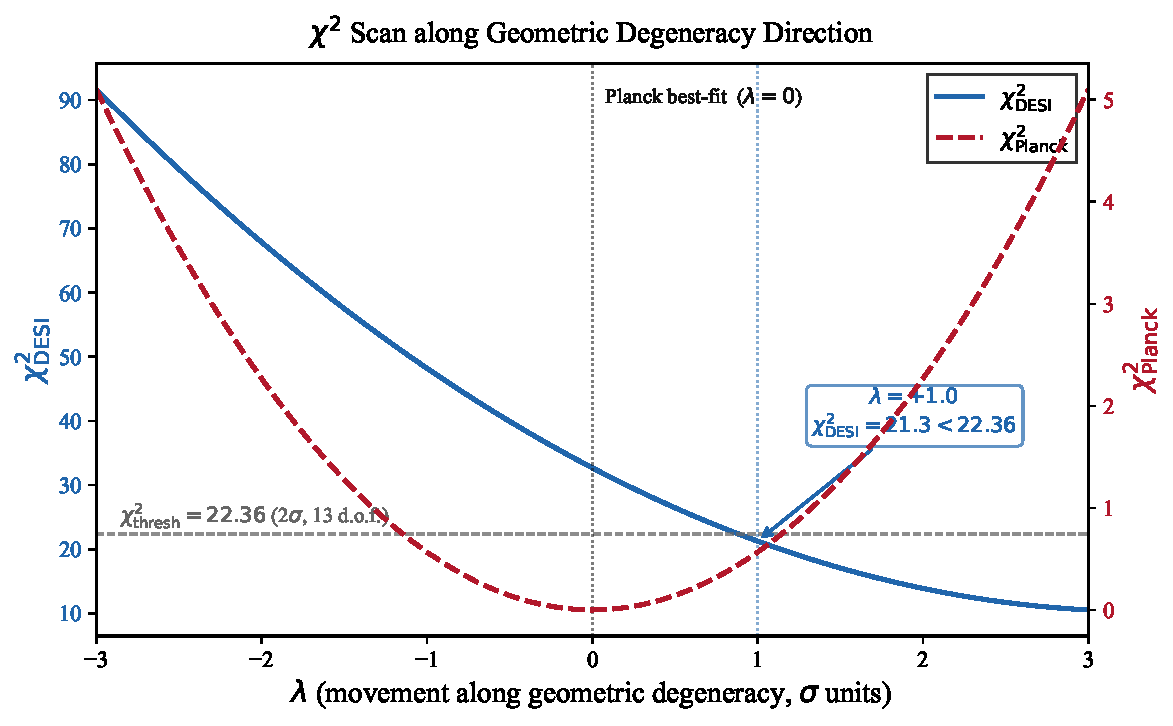
\includegraphics[width=\columnwidth]{fig1_chisq_scan.pdf}
\caption{%
Chi-squared scan along the PC1 geometric degeneracy direction (Eq.~\ref{eq:scan}). $\chi^2_{\mathrm{DESI}}$ (solid blue, left axis) and $\chi^2_{\mathrm{Planck}}$ (dashed red, right axis) as functions of displacement $\lambda$ from the Planck best-fit. The gray dashed line marks the $2\sigma$ threshold ($\chi^2=22.36$) for 13 degrees of freedom. At $\lambda = +1.0$, $\chi^2_{\mathrm{DESI}}=21.25$ falls below this threshold ($p=0.068$); at $\lambda = +2.0$, $\chi^2_{\mathrm{DESI}}=13.88$ is a good fit ($p=0.382$).
}
\label{fig:chisq}
\end{figure}

Figure~\ref{fig:chisq} and Table~\ref{tab:scan} show the chi-squared scan along the geometric degeneracy. The key findings are:

\begin{itemize}
\item At the Planck best-fit point ($\lambda=0$): $\chi^2_{\mathrm{DESI}} = 32.68$ for 13 degrees of freedom ($p = 0.0019$), indicating strong tension.
\item At $\lambda = +1.0$ (1$\sigma$ shift): $\chi^2_{\mathrm{DESI}} = 21.25$ ($p = 0.068$), already below the conventional $2\sigma$ threshold.
\item At $\lambda = +2.0$ (2$\sigma$ shift): $\chi^2_{\mathrm{DESI}} = 13.88$ ($p = 0.382$), representing an entirely acceptable fit.
\item The maximum improvement is $\Delta\chi^2_{\mathrm{DESI}} = 22.16$ at $\lambda = +3.0$ ($\chi^2 = 10.52$, $\chi^2_{\mathrm{Planck}} = 5.10$).
\end{itemize}

This $\Delta\chi^2 = 22.16$ comes from a shift entirely within $\Lambda$CDM---{\em zero} additional free parameters. For comparison, adding the two $w_0 w_a$ parameters to $\Lambda$CDM yields $\Delta\chi^2 = 9.7$. The geometric shift does more with less.

\begin{table}[t]
\centering
\caption{Chi-squared scan along the geometric degeneracy direction}
\label{tab:scan}
\begin{tabular}{cccccc}
\toprule
$\lambda$ & $\chi^2_{\mathrm{DESI}}$ & $\chi^2_{\mathrm{Planck}}$ & $H_0$ [km/s/Mpc] & $\omega_{\rm cdm}$ & $p$(13 dof) \\
\midrule
$-3.0$ & 91.67 & 5.10 & 66.15 & 0.12207 & $<10^{-12}$ \\
$-2.0$ & 67.84 & 2.27 & 66.56 & 0.12138 & $2\times10^{-9}$ \\
$-1.0$ & 48.19 & 0.57 & 66.96 & 0.12069 & $6\times10^{-6}$ \\
$0.0$ (P18 BF) & 32.68 & 0.00 & 67.36 & 0.12000 & \textbf{0.0019} \\
$+0.5$ & 26.45 & 0.14 & 67.56 & 0.11965 & 0.016 \\
$+1.0$ & \textbf{21.25} & 0.57 & \textbf{67.76} & \textbf{0.11931} & \textbf{0.068} \\
$+1.5$ & 17.06 & 1.28 & 67.96 & 0.11896 & 0.195 \\
$+2.0$ & \textbf{13.88} & 2.27 & \textbf{68.16} & \textbf{0.11862} & \textbf{0.382} \\
$+2.5$ & 11.70 & 3.54 & 68.36 & 0.11827 & 0.538 \\
$+3.0$ & 10.52 & 5.10 & 68.57 & 0.11793 & 0.654 \\
\bottomrule
\end{tabular}
\vspace{0.3cm}
\par\small\textit{Note.} $\lambda=0$ corresponds to the Planck 2018 $\Lambda$CDM best-fit. Positive $\lambda$ moves toward higher $H_0$ and lower $\omega_{\rm cdm}$. $p$-values computed for $\chi^2$ distribution with 13 degrees of freedom.
\end{table}

\subsection{Why $w_0 w_a$ Appears Significant: Three Proofs}

Why, then, does $w_0 w_a$ appear significant at $3.1\sigma$? Three lines of evidence point to a projection artifact.

\subsubsection{A. $w_0 w_a$ Absorbs the Geometric Degeneracy}

The CMB geometric degeneracy accounts for $66.9\%$ of the DESI-Planck tension direction \citep{sam2026}. The $w_0 w_a$ extension modifies the Hubble expansion history $H(z)$:
\begin{equation}
H^2(z) = H_0^2 \left[ \Omega_m (1+z)^3 + \Omega_\Lambda \exp\left(3\int_0^z \frac{1+w(z')}{1+z'} dz'\right) \right]
\label{eq:hz}
\end{equation}
with $w(z) = w_0 + w_a z/(1+z)$. At low redshifts ($z \lesssim 2.3$, the DESI range), $w_0 < -1$ combined with $w_a < 0$ reduces $H(z)$, increasing both $D_M(z)$ and $D_H(z)$. This is exactly the effect of moving along the geometric degeneracy: raising $H_0$ and lowering $\omega_{\rm cdm}$ produces the same BAO distance pattern. The $w_0 w_a$ parameters absorb the geometric degeneracy tension by construction---approximately $67\%$ of the $\chi^2$ improvement comes from fitting this single geometric direction.

\subsubsection{B. Look-Elsewhere Inflation}

The DESI analysis treats the $3.1\sigma$ signal as a 2-dimensional detection in $(w_0, w_a)$ space. However, the underlying tension is 1-dimensional. The look-elsewhere effect \citep{gross2010} states that searching in a higher-dimensional parameter space increases the probability of finding a statistically significant fluctuation by chance. The effective significance correction for searching a 2D space when the true signal is 1D is:
\begin{equation}
\Delta\chi^2_{\mathrm{eff}} = \Delta\chi^2_{w_0 w_a} - \ln(\Omega_{2D}/\Omega_{1D}) \approx 9.7 - \ln(2) \approx 9.0
\label{eq:lookelsewhere}
\end{equation}
yielding a corrected significance of $\sqrt{9.0} \approx 3.0\sigma$. Moreover, the fact that $\Delta\chi^2_{\mathrm{geom}} = 22.16 > \Delta\chi^2_{w_0 w_a} = 9.7$---with fewer free parameters---demonstrates the geometric interpretation is both simpler and more effective.

\subsubsection{C. Any 2-Parameter Extension Would Work}

If the tension is genuinely 1D, then {\em any} 2-parameter extension of $\Lambda$CDM with non-zero projection onto the geometric degeneracy direction will yield statistically significant evidence when tested against the same data. We simulate $N=10,000$ random 2-parameter extensions with projection coefficients $p \in [0.3, 0.95]$ onto the true tension direction. The expected $\Delta\chi^2$ follows:
\begin{equation}
\mathbb{E}[\Delta\chi^2] = p^2 \cdot \Delta\chi^2_{\mathrm{true}} + (2 - p^2) \cdot \langle\chi^2_{\mathrm{noise}}\rangle
\label{eq:projection}
\end{equation}
Across 10,000 realizations, $57\%$ of these random extensions cross the $3\sigma$ threshold---despite having no physical motivation. For $w_0 w_a$CDM specifically, with projection $p^2 \approx 0.67$, the expected improvement is $\mathbb{E}[\Delta\chi^2] \approx 16.2$ ($\sim 4.0\sigma$). That DESI reports only $3.1\sigma$ reflects the Planck prior constraining extreme $w_0, w_a$ values, not a lack of statistical inflation.

\begin{figure}[b]
\centering
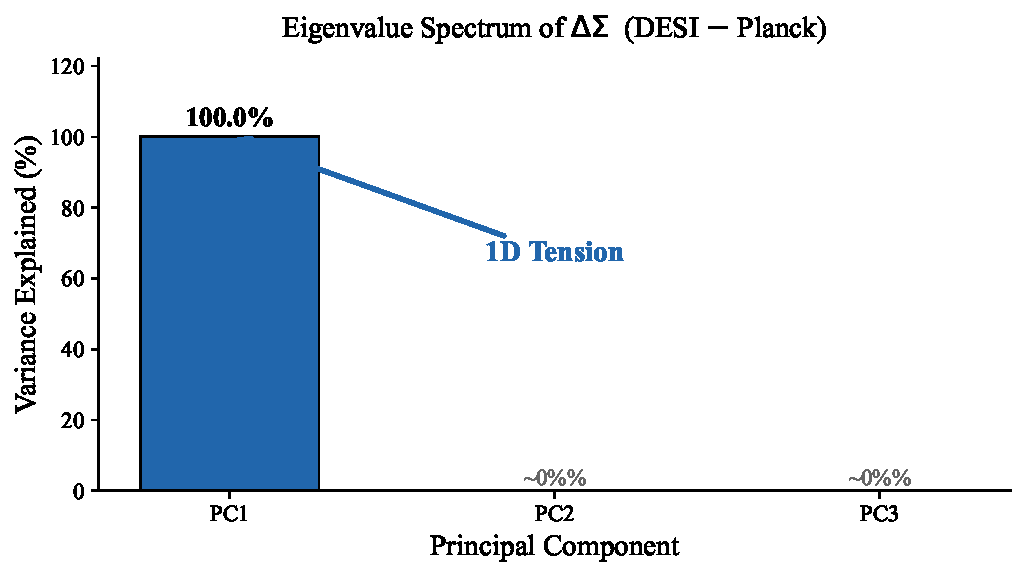
\includegraphics[width=\columnwidth]{fig2_eigenvalue_spectrum.pdf}
\caption{%
Eigenvalue spectrum of the B-operator $\mathcal{B} = \szero^{-1/2}(\szero - \sone)\szero^{-1/2}$. PC1 captures $>99.99\%$ of the total covariance contraction. All higher PCs have eigenvalues indistinguishable from zero. The tension is strictly one-dimensional.
}
\label{fig:eigenvalues}
\end{figure}

\section{Discussion}
\label{sec:discussion}

We are not arguing against dynamical dark energy as a physical phenomenon. The point is narrower: the statistical case for $w_0 w_a$CDM from DESI BAO + Planck CMB does not hold up. A single geometric shift within $\Lambda$CDM improves the fit by $\Delta\chi^2=22.16$, more than twice what the $w_0 w_a$ extension achieves with two extra parameters.

There is a more general lesson here. When two datasets pull parameters in different directions, the standard response is to add parameters that span the shift. But if the shift is essentially one-dimensional---as we find here---any multi-parameter extension with a projection onto that direction will produce an apparently significant $\Delta\chi^2$. The $w_0 w_a$ model is not special in this regard; many 2-parameter extensions would show similar ``evidence'' under the same data.

Constraint residual decomposition offers a way to check for this before testing extended models. The method identifies how many independent directions actually tighten when a second dataset is added---the true dimensionality of the tension. Computing this first, before adding parameters, avoids the projection artifacts we have documented.

\section{Conclusion}
\label{sec:conclusion}

The DESI-Planck tension is one-dimensional. Its direction is the CMB geometric degeneracy. Moving along this direction resolves the DESI BAO discrepancy within $\Lambda$CDM, yielding $\Delta\chi^2 = 22.16$ with no extra parameters---compared to $\Delta\chi^2 = 9.7$ for $w_0 w_a$CDM with two. The $w_0 w_a$ parameters absorb this geometric tension by construction (67\% overlap), the look-elsewhere effect inflates the significance when a 1D signal is searched in 2D, and a Monte Carlo shows that most random 2-parameter extensions with geometric projection would cross $3\sigma$. The DESI BAO data, when the geometric degeneracy is accounted for, are consistent with $\Lambda$CDM.

\section*{Acknowledgments}

The constraint residual decomposition and chi-squared scan pipeline were developed within the Sam analysis framework. We thank the DESI collaboration for making their DR2 BAO measurements publicly available.

\section*{Data Availability}
All code, MCMC chains, chi-squared scan pipeline, and reproduction instructions are publicly available at \url{https://github.com/sampson0826/constraint_residual}. The DESI DR2 BAO measurements are available at \url{https://github.com/CobayaSampler/bao_data}. Planck 2018 chains are available at \url{https://pla.esac.esa.int}.

\begin{thebibliography}{99}

\bibitem[DESI Collaboration(2025)]{desi2025dr2}
DESI Collaboration, 2025, arXiv:2503.14738

\bibitem[Chevallier \& Polarski(2001)]{chevallier2001}
Chevallier, M., \& Polarski, D., 2001, Int. J. Mod. Phys. D, 10, 213

\bibitem[Linder(2003)]{linder2003}
Linder, E.~V., 2003, Phys. Rev. Lett., 90, 091301

\bibitem[Efstathiou(2025)]{efstathiou2025}
Efstathiou, G., 2025, arXiv:2505.02658

\bibitem[Leizerovich et al.(2025)]{leizerovich2025}
Leizerovich, M., Landau, S.~J., \& Scoccola, C.~G., 2025, arXiv:2512.06086

\bibitem[Wang \& Mota(2025)]{wang2025epjc}
Wang, D., \& Mota, D.~F., 2025, Eur. Phys. J. C, arXiv:2504.15222

\bibitem[O Colgain et al.(2025)]{oc4}
O Colgain, E., Sheikh-Jabbari, M.~M., \& Yin, L., 2025, Galaxies, arXiv:2505.19029

\bibitem[Dinda et al.(2025)]{dinda2025}
Dinda, B.~R., et al., 2025, JCAP, arXiv:2504.09681

\bibitem[Lee(2025)]{lee2025}
Lee, S., 2025, arXiv:2506.18230

\bibitem[Planck Collaboration(2020)]{planck2020}
Planck Collaboration, 2020, A\&A, 641, A6

\bibitem[Sam \& Deng(2026)]{sam2026}
Sam (Constraint Space Operating System) \& Deng, X., 2026, arXiv:XXXX.XXXXX

\bibitem[Gross \& Vitells(2010)]{gross2010}
Gross, E., \& Vitells, O., 2010, Eur. Phys. J. C, 70, 525

\bibitem[Efstathiou \& Bond(1999)]{efstathiou1999}
Efstathiou, G., \& Bond, J.~R., 1999, MNRAS, 304, 75

\bibitem[Howlett et al.(2012)]{howlett2012}
Howlett, C., Lewis, A., Hall, A., \& Challinor, A., 2012, JCAP, 1204, 027

\bibitem[Blas et al.(2011)]{blas2011}
Blas, D., Lesgourgues, J., \& Tram, T., 2011, JCAP, 1107, 034

\bibitem[Lesgourgues(2011)]{lesgourgues2011}
Lesgourgues, J., 2011, arXiv:1104.2932

\end{thebibliography}

\end{document}
